%%%%%%%%%%%%%%%%%%%%%%%%%%%%%%%%%%%%%%%%%%%%%%%%%%
%% Bachelor's & Master's Thesis Template        %%
%% Copyleft by Dawid Weiss & Marta Szachniuk    %%
%% Faculty of Computing and Telecommunication   %%
%% Poznan University of Technology, 2020        %%
%%%%%%%%%%%%%%%%%%%%%%%%%%%%%%%%%%%%%%%%%%%%%%%%%%


% Szkielet dla pracy licencjackiej pisanej w języku polskim.

\documentclass[english,engineering,a4paper,oneside]{ppfcmthesis}


\usepackage[utf8]{inputenc}
\usepackage[OT4]{fontenc}
\usepackage{amsmath}
\usepackage{tikz}
\usepackage{subcaption}
\usepackage{stmaryrd}
\usepackage{listings}
\usepackage{multirow}

% Define the JSON style
\lstdefinelanguage{json}{
  basicstyle=\ttfamily\small,
  commentstyle=\color{green},
  keywordstyle=\color{blue},
  numberstyle=\tiny\color{gray},
  stringstyle=\color{red},
  breaklines=true,
  showstringspaces=false,
  tabsize=2
}

%--------------------------------------
% Strona tytułowa
%--------------------------------------

% Autorzy pracy, jeśli jest ich więcej niż jeden
% wstaw między nimi separator \and
\author{%
   Maciej Iwaszkiewicz \album{148275} \and 
   Kamil Kałużny \album{148121} \and
   Jan Krenz \album{148144} \and 
   Piotr Wojsznis \album{147414} } 
\authortitle{}                                % Do not change.

\title{A machine learning system for short-term weather prediction}

% Your supervisor comes here.
\ppsupervisor{prof. PP ~dr hab.~inż.~Wojciech Kotłowski} 

% Year of final submission (not graduation!)
\ppyear{2024}                                 


\begin{document}

% Front matter starts here
\frontmatter\pagestyle{empty}%
\maketitle\cleardoublepage%


%--------------------------------------
% Spis treści
%--------------------------------------

\pagenumbering{Roman}\pagestyle{ppfcmthesis}%
\tableofcontents* 
\cleardoublepage % Zaczynamy od nieparzystej strony

%--------------------------------------
% Rozdziały
%--------------------------------------

%Najwygodniej jeśli każdy rozdział znajduje się w oddzielnym pliku
\mainmatter%

\chapter{Introduction}

\section{Abstract}
The drastically changing climate in recent times has led to a significant increase in interest in the research related to modeling weather and meteorological phenomena. Machine learning scientists are trying to surpass the previous state-of-the-art methods in this field, that leverage numerical computations. 

Given that weather states can be interpreted as highly complex dynamical systems, utilizing deep learning methods appears reasonable due to their flexibility and proficiency in handling complex data. These attributes position deep learning as a potentially successful set of techniques in this field.

Attributable to the above statements, in our work, we present the forecasting capabilities of straightforward methods of classical machine learning as well as design a more complex model based on graph neural networks. In addition, we compare the quality of distinct solutions and create a full system with a mobile application presenting the predictive skills of the created architecture. 

Finally, in a notable achievement, we integrate our top-performing solution with an arbitrarily selected approach from the numerical weather prediction paradigm -- improving its predictive performance. This accomplishment underscores the potential of enhancing numerical methods through integration with advanced deep learning solutions.

\section{Motivation}
At the present rate of progress, machine learning methods are applied and often give great promise in almost all areas of our lives. With this work, we would like to add our contribution to this issue with regard to the problem of short-term weather prediction. Until now, the models obtaining the finest results in this area belong to the "Numerical Weather Prediction" (NWP) family. An example of such a solution might be IFS \cite{ECMWFIFS}, incorporated by EMCWF -- "European Centre for Medium-Range Weather Forecasts". Their most significant weakness is that they are computationally very expensive. Supercomputers generating serious carbon footprints are often needed for the model to run effectively. These models attempt to solve complex differential equations with very high precision. Moreover, their prediction time is often very long. 
For this reason, machine learning-based solutions from the "Machine Learning Weather Prediction" (MLWP) family are becoming increasingly popular, therefore we want to focus on them in our work. The particular example that caused us to get interested in the topic was the publication of a paper "Learning skillful medium-range global weather forecasting" \cite{lam2023graphcast} about GraphCast, further described in Section \ref{sec:graphcast}. 

\section{Goals}
One of the main goals is to implement various machine learning methods for the examined task and to extensively analyze their predictive capabilities depending on the sizes of the model's input and output size as well as architectural details, such as those related to the number of layers in the neural network. Additionally, we aim to obtain sufficient results that allow us to support the thesis that graph neural networks and generally machine learning approaches for weather prediction tasks are promising and worth developing. Furthermore, as a practical application of our research, we aspire to create a mobile application that will display accurate and the latest possible weather predictions derived from our best-performing model.

\section{Scope}
\subsection{Dataset}
During our work, we have used the Copernicus Climate Change Service (C3S) Climate Data Store (CDS) "ERA5 hourly data on single levels from 1940 to present" dataset \cite{ERA5}. It contains regularly updated hourly global weather data from 1940 to present -- usually with about 5 days of latency. It is provided by the European Centre for Medium-Range Weather Forecasts (EMCWF) and combines vast amounts of historical observations into global estimates using advanced modelling and data assimilation systems. There are many atmospheric, ocean-wave and land-surface quantities inside, however we have decided to focus on 6 features (Table \ref{tab:data_features}).

\begin{table}[!ht]
\centering
\begin{tabular}{|c|c|c|}
     \hline
     Symbol & Quantity & Unit \\
     \hline
     t2m & Temperature at 2m above ground & $^{\circ}$C \\
     sp & Surface pressure & hPa \\
     tcc & Total cloud cover & (0 - 1) \\
     u10 & 10m U wind component & $m/s$ \\
     v10 & 10m V wind component & $m/s$ \\
     tp & Total precipitation & mm \\
     \hline
     lsm & Land-sea mask (not predicted) & (0 - 1) \\
     z & Geopotential (not predicted) & $m^2/s^2$ \\
     \hline
\end{tabular}
\caption{Weather features we considered. Some of the units differ from those provided in the dataset. These have been converted for our convenience}
\label{tab:data_features}
\end{table}

These features were determined by us to be the most useful, and during our proceedings the models will attempt to accurately predict them. Apart from the self-explanatory, the U and V wind components represent the speed of wind moving towards the east and the north respectively. We also used 2 other quantities that provide additional information to our neural network models -- a binary land-sea mask and geopotential, which is the gravitational potential energy of a unit mass, which can be interpreted as a measure of orography. These two features are never predicted.

During our work, we have used many different timespans of the dataset, always from 2018 - 2023. Most commonly, we used 2019 - 2022, since that can be easily divided into the training, validation, and test datasets, with each having a full year worth of data. More details on our use of the dataset can be found in Section \ref{chap:dataset}.

\subsection{Models}
The research part of our thesis will be primarily devoted to the implementation and analysis of machine learning models. Based on the literature review, we will attempt to leverage the techniques used in examined state-of-the-art solutions into our primary model. For all implemented solutions, we will conduct numerous experiments checking, among other things, the quality of forecasting depending on the length of the model's input sequence (i.e., the past time steps the model has access to) and also how the models perform with increasing forecasting horizon (the number of forecasted future time steps). In addition, to obtain the estimation of optimal performance per model, we will perform hyperparameter optimizations for each. Lastly, we will compare the quality of prediction with the ERA5 dataset adopted as ground truth weather states and the topline solution, based on the Numerical Weather Prediction paradigm. 
% Survey multiple machine learning models and a lighter version of GraphCast architecture. Perform experiments, compare results with ground truth weather states dataset ERA5 and SOTA/topline solution based on fluid dynamics or other related to Numerical Weather Prediction approach.

\subsection{App}
In this section of the thesis, we will focus on another aspect of our machine learning system for short-term weather prediction – the mobile application and its integration with an API. Our primary goal is to examine the functionality and structure of the application, serving as a conduit for users to access predictions generated by our model.

The application plays a pivotal role in facilitating communication with our machine learning model through an Application Programming Interface (API). This enables users to access predictive insights seamlessly, providing an accessible means to leverage advanced weather forecasting. Utilizing Android Studio, Google's official integrated development environment for Android, the mobile application is designed to offer a user-friendly experience. The emphasis is not only on the predictions but also on ensuring the application's overall functionality and structure allow users to navigate and interpret information effortlessly.

\section{Methodology}

The most crucial foundation of any project developed within a group is effective communication and planning of undertaken actions. Central to our approach is the adoption of Agile principles, emphasizing adaptability and collaboration throughout the project's lifecycle. The fluidity of live-coding sessions aligns with Agile principles, ensuring that our development process remains responsive to evolving requirements and feedback. Code is stored and shared through GitHub, providing a centralized repository for version control and collaborative code management. These methods contributed to the flexibility and responsiveness crucial for successfully navigating the challenges inherent in the development of a complex machine learning system. Furthermore, we utilized the mathcha.io tool to generate figures in TikZ language \cite{mathcha}.

\section{Author-Specific Contributions}
\begin{itemize}
    \item Maciej Iwaszkiewicz -- Exponential smoothing development and testing. Neural network infrastructure: help with developing the training pipeline, implementing the Spatio-Temporal Embedder, development and implementation of the U-net model, including a separate Trainer and data processor subclass. Hyperparameter optimization, analysis: running and analysing the HPO for the U-net. App: help with creating the API. Containerizing, deployment, and running of the API. Miscellaneous: working with date and time representations
    \item Kamil Kałużny -- Baselines framework development: all functionality, including the autoregressive evaluation and neighbor extension, implementing naive baseline, both linear regressions and gradient boosting trees. Neural network infrastructure: building training and evaluating pipelines -- Trainer, designing Spatio-Temporal Embedder with feature engineering methods, and implementing the rest of the Graph Neural Network components and spatial mapping. Research and review: conducted literature review, explored and tested multiple GNN solutions and regularization techniques for optimal performance, dataset analysis, and visualizations. Project coordination: scrum mastering, providing thesis syllabus, outlining plans for most of the performance analysis and hyperparameters optimization. Experiments and integration: executing all experiments, integrating within the project cartopy maps and TIGGE solution.
    \item Jan Krenz -- Development of a mobile application - designing the interface and programming the entire solution, designing icons representing weather conditions, and the application logo. Writing the source code for the API responsible for processing the model prediction results so that it is compatible with the application.
    \item Piotr Wojsznis -- Hyperparameter optimization: development of the pipeline responsible for obtaining the optimized hyperparameters, and running it.  Analysis: design and creation of pipeline for obtaining, saving and plotting analysis results. Baseline development: additional help in the development process. Map Creation: developing functions for quality map representation of model outputs. TIGGE: development of functions for processing and evaluating data from TIGGE.
\end{itemize}


\chapter{Theoretical introduction}
	
\section{Problem introduction}
 Theoretical introduction to a problem and mathematical concepts, literature review.... \\
 
\noindent General task is to predict a weather state $\Omega_t$, observed at a timestamp $t$, given $s$ steps from the past, which are essentially previous weather states: $(\Omega_{t-1}, ..., \Omega_{t-s})$. We define $\Omega_t$ as a tensor of a shape: (latitude span, longitude span, features), therefore our complete input data would be 4-dimensional with additional dimension for a time \footnote{To be precise, for neural network based solutions it will be 5-dimensional due to the usage of batches.}. Spatial span was selected so as to cover the border of the whole of Poland and some of its neighbors. More details regarding data are discussed in dataset chapter~\ref{chap:dataset}. High-level spatio-temporal prediction framework is presented at Figure~\ref{fig:in_out}. \\

\noindent Forecasting performance would be evaluating by objective function:
\[
    \mathcal{L}(\hat{X}, X)
\]


\newpage
\subsection{Naming conventions and general prediction framework}
 For further convenience, we propose a general naming convention. 
 \begin{table}[!h]
    \centering
     \begin{tabular}{|c|c|}
        \hline
        Symbol & Description \\
        \hline
        $\mathbf{f}$ & Set of features: $(f_1,..., f_n)$ \\
        $s$ & Number of past steps \\
        $h$ & Forecasting horizon \\
        $\Omega$ & Weather state for all features \\
        $X_t$ & $\Omega$ for timestamp t\\
        $\mathbf{X}$ & $s$-element set of $\Omega$  \\
        $\hat{Y_t}$ & Prediction of $\Omega$ for timestamp t \\
        $\mathbf{\hat{Y}}$ & $h$-element set of predicted $\Omega$ \\
        $\hat{y_t}^{f_j}$ & Prediction of $\Omega$ for timestamp t and feature $f_j$ \\
        \hline
    \end{tabular}
    \caption{General conventions}
 \end{table}
 
 
%% \noindent We define a $\Phi$ as a set of baseline models that consist of: 
\begin{table}[!h]
    \centering
    \begin{tabular}{|c|c|}
        \hline
        Model Notation & Model Description \\
        \hline
        $\Phi_{es}$  & Exponential Smoothing \\
        $\Phi_{slr}$ & Simple Linear Regression \\
        $\Phi_{lr}$  & Linear Regression \\
        $\Phi_{gb}$ & Gradient Boosting Trees \\
        \hline
    \end{tabular}
\caption{Model conventions}
\end{table}
 
%% \noindent Additionally, due to the fact that model $\Phi_i$ consist of independent models that predicts single feature $f_j$ of a weather state, we can divide it into: 
 
 \noindent It is crucial to emphasize the fact that the scale of values of distinct features is diverse. Therefore, we define a model $\Phi_i$ as a collection of independent sub-models, each exclusively responsible for predicting distinct feature $f_j$. This solution was proposed to avoid situations in which the statistical dispersion of one feature might influence the prediction of another feature.  
 \[
 \Phi_{i} = (\Phi_{i}^{f_1}, ..., \Phi_{i}^{f_n})
 \]
 In further considerations, we will use a term: sub-models for each of $\Phi_{i}^{f_j}$.


\begin{figure}[!h]



\tikzset{every picture/.style={line width=0.75pt}} %set default line width to 0.75pt        

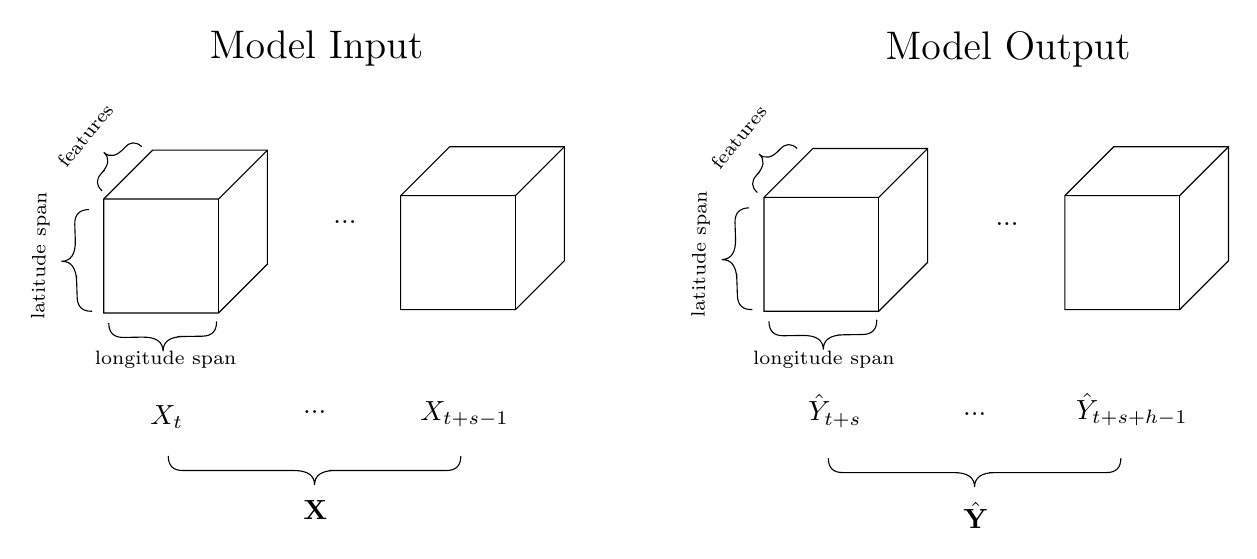
\begin{tikzpicture}[x=0.75pt,y=0.75pt,yscale=-1,xscale=1]
%uncomment if require: \path (0,389); %set diagram left start at 0, and has height of 389

%Shape: Cube [id:dp2816308175879604] 
\draw   (58.25,114.54) -- (81.78,91.01) -- (137.08,91.01) -- (137.08,145.91) -- (113.55,169.44) -- (58.25,169.44) -- cycle ; \draw   (137.08,91.01) -- (113.55,114.54) -- (58.25,114.54) ; \draw   (113.55,114.54) -- (113.55,169.44) ;
%Shape: Brace [id:dp4309828249836092] 
\draw   (76.63,89.37) .. controls (73.72,86.74) and (70.94,86.88) .. (68.31,89.8) -- (68.31,89.8) .. controls (64.55,93.97) and (61.21,94.73) .. (58.29,92.1) .. controls (61.21,94.73) and (60.79,98.13) .. (57.03,102.29)(58.72,100.42) -- (57.03,102.29) .. controls (54.4,105.21) and (54.54,107.99) .. (57.45,110.62) ;
%Shape: Brace [id:dp7756675475750493] 
\draw   (51.06,119.6) .. controls (46.39,119.75) and (44.14,122.16) .. (44.29,126.83) -- (44.53,134.35) .. controls (44.75,141.01) and (42.53,144.42) .. (37.86,144.57) .. controls (42.53,144.42) and (44.97,147.67) .. (45.19,154.34)(45.09,151.34) -- (45.43,161.86) .. controls (45.58,166.52) and (47.99,168.77) .. (52.66,168.62) ;
%Shape: Brace [id:dp612063156099937] 
\draw   (60.65,174.34) .. controls (60.72,179.01) and (63.09,181.3) .. (67.76,181.23) -- (76.73,181.09) .. controls (83.4,180.98) and (86.77,183.26) .. (86.84,187.93) .. controls (86.77,183.26) and (90.06,180.88) .. (96.73,180.78)(93.73,180.82) -- (105.71,180.64) .. controls (110.38,180.57) and (112.67,178.2) .. (112.6,173.53) ;
%Shape: Cube [id:dp42835259632452516] 
\draw   (201.31,112.9) -- (224.84,89.37) -- (280.14,89.37) -- (280.14,144.28) -- (256.61,167.81) -- (201.31,167.81) -- cycle ; \draw   (280.14,89.37) -- (256.61,112.9) -- (201.31,112.9) ; \draw   (256.61,112.9) -- (256.61,167.81) ;
%Shape: Brace [id:dp07592439753840141] 
\draw   (89.33,238.35) .. controls (89.33,243.02) and (91.66,245.35) .. (96.33,245.35) -- (149.81,245.35) .. controls (156.48,245.35) and (159.81,247.68) .. (159.81,252.35) .. controls (159.81,247.68) and (163.14,245.35) .. (169.81,245.35)(166.81,245.35) -- (223.29,245.35) .. controls (227.96,245.35) and (230.29,243.02) .. (230.29,238.35) ;
%Shape: Cube [id:dp7110500253196546] 
\draw   (376.35,113.72) -- (399.88,90.19) -- (455.18,90.19) -- (455.18,145.09) -- (431.65,168.62) -- (376.35,168.62) -- cycle ; \draw   (455.18,90.19) -- (431.65,113.72) -- (376.35,113.72) ; \draw   (431.65,113.72) -- (431.65,168.62) ;
%Shape: Brace [id:dp86120893233015] 
\draw   (392.33,90.19) .. controls (389.42,87.56) and (386.64,87.7) .. (384.01,90.62) -- (384.01,90.62) .. controls (380.25,94.78) and (376.91,95.54) .. (373.99,92.91) .. controls (376.91,95.54) and (376.49,98.94) .. (372.73,103.11)(374.42,101.24) -- (372.73,103.11) .. controls (370.1,106.02) and (370.24,108.8) .. (373.15,111.43) ;
%Shape: Brace [id:dp9673653209625941] 
\draw   (369.15,118.79) .. controls (364.49,118.94) and (362.24,121.34) .. (362.39,126.01) -- (362.63,133.53) .. controls (362.85,140.2) and (360.63,143.6) .. (355.96,143.75) .. controls (360.63,143.6) and (363.07,146.86) .. (363.28,153.52)(363.19,150.52) -- (363.53,161.04) .. controls (363.68,165.71) and (366.09,167.96) .. (370.75,167.81) ;
%Shape: Brace [id:dp9113296386668477] 
\draw   (378.74,173.53) .. controls (378.81,178.2) and (381.18,180.49) .. (385.85,180.42) -- (394.83,180.27) .. controls (401.5,180.17) and (404.87,182.45) .. (404.94,187.12) .. controls (404.87,182.45) and (408.16,180.07) .. (414.83,179.96)(411.83,180.01) -- (423.8,179.82) .. controls (428.47,179.75) and (430.76,177.38) .. (430.69,172.71) ;
%Shape: Cube [id:dp35039842919754816] 
\draw   (521.31,112.9) -- (544.84,89.37) -- (600.14,89.37) -- (600.14,144.28) -- (576.61,167.81) -- (521.31,167.81) -- cycle ; \draw   (600.14,89.37) -- (576.61,112.9) -- (521.31,112.9) ; \draw   (576.61,112.9) -- (576.61,167.81) ;
%Shape: Brace [id:dp3763157845274283] 
\draw   (407.33,239.35) .. controls (407.33,244.02) and (409.66,246.35) .. (414.33,246.35) -- (467.81,246.35) .. controls (474.48,246.35) and (477.81,248.68) .. (477.81,253.35) .. controls (477.81,248.68) and (481.14,246.35) .. (487.81,246.35)(484.81,246.35) -- (541.29,246.35) .. controls (545.96,246.35) and (548.29,244.02) .. (548.29,239.35) ;

% Text Node
\draw (33.24,96.31) node [anchor=north west][inner sep=0.75pt]  [rotate=-309.39,xslant=-0.03] [align=left] {{\scriptsize features}};
% Text Node
\draw (79.43,212.59) node [anchor=north west][inner sep=0.75pt]    {$X_{t}$};
% Text Node
\draw (167.65,123.51) node [anchor=north west][inner sep=0.75pt]   [align=left] {...};
% Text Node
\draw (21.86,173.65) node [anchor=north west][inner sep=0.75pt]  [rotate=-270.99] [align=left] {{\scriptsize latitude span}};
% Text Node
\draw (52.73,186.5) node [anchor=north west][inner sep=0.75pt]   [align=left] {{\scriptsize longitude span}};
% Text Node
\draw (209.49,210.96) node [anchor=north west][inner sep=0.75pt]    {$X_{t+s-1}$};
% Text Node
\draw (153.04,215.29) node [anchor=north west][inner sep=0.75pt]   [align=left] {...};
% Text Node
\draw (153.16,258.53) node [anchor=north west][inner sep=0.75pt]    {$\mathbf{X}$};
% Text Node
\draw (433.72,32.89) node [anchor=north west][inner sep=0.75pt]   [align=left] {{\Large Model Output}};
% Text Node
\draw (108.05,32.26) node [anchor=north west][inner sep=0.75pt]   [align=left] {{\Large Model Input}};
% Text Node
\draw (348.14,97.12) node [anchor=north west][inner sep=0.75pt]  [rotate=-309.39,xslant=-0.03] [align=left] {{\scriptsize features}};
% Text Node
\draw (339.95,172.84) node [anchor=north west][inner sep=0.75pt]  [rotate=-270.99] [align=left] {{\scriptsize latitude span}};
% Text Node
\draw (369.83,186.68) node [anchor=north west][inner sep=0.75pt]   [align=left] {{\scriptsize longitude span}};
% Text Node
\draw (486.65,124.51) node [anchor=north west][inner sep=0.75pt]   [align=left] {...};
% Text Node
\draw (396.43,207.59) node [anchor=north west][inner sep=0.75pt]    {$\hat{Y}_{t+s}$};
% Text Node
\draw (525.49,206.96) node [anchor=north west][inner sep=0.75pt]    {$\hat{Y}_{t+s+h-1}$};
% Text Node
\draw (471.04,216.29) node [anchor=north west][inner sep=0.75pt]   [align=left] {...};
% Text Node
\draw (471.16,259.53) node [anchor=north west][inner sep=0.75pt]    {$\hat{\mathbf{Y}}$};


\end{tikzpicture}


\caption{Spatio-Temporal prediction framework}  \label{fig:in_out} 


\end{figure}


\noindent Take into account the fact that this framework may differ when applying techniques such as grid neighbors~\ref{chap:neighbors} or using constants encodings~\ref{chap:feat_eng}. Details regarding those differences are explained deeply in subsequent chapters.

 \newpage
 
 \subsection{Literature review}
 After stating the problem we want to shortly inspect current research and results in this field... \\
Short review of quality papers related to this problem; explanation of what was already achieved in this task - SOTA solutions, especially emphasizing GraphCast paper; what we want to reproduce or compare ourself with. \\
\noindent Maybe start with: ~\cite{WFConsiderations}
MetNet, FourCastNet, GraphCast, and PanGu are state-of-the-art methods in the field of weather prediction.

\section{Explored techniques}
 \subsection{Autoregression}
 \noindent Each baseline model is designed to forecast the entire weather state for subsequent timestamp, with the forecasting horizon set at one. Therefore, when employing our models for short-term prediction tasks exceeding a few timestamps into the future, the autoregressive approach is commonsensical. \\ \\
 
 \noindent We denote model input as $\mathbf{X}$, a tensor of $s$ weather states: 
 \[
 \mathbf{X} = (X_{t}, ..., X_{t+s-1})
 \]
 and output of a model as $\mathbf{\hat{Y}}$, which consist of $h$ forecasted states:
 \[
 \mathbf{\hat{Y}} = (\hat{Y}_{t+s}, ..., \hat{Y}_{t+s+h-1})
 \]
 
 \noindent Autoregressive prediction is $h$-steps process such that:
 \begin{flalign*}
    &\hat{Y}_{t+s} = \Phi_{i}(X_{t}, ..., X_{t+s-1}) \\
    &\hat{Y}_{t+s+1} = \Phi_{i}(X_{t+1}, ..., X_{t+s-1}, \hat{Y}_{t+s}) \\
    &\vdots \\
    &\hat{Y}_{t+s+h-1} = \Phi_{i}(X_{t+h-1}, ...,  \hat{Y}_{t+s+h-3}, \hat{Y}_{t+s+h-2})
 \end{flalign*}

 \noindent Therefore, by simplifying:
 \[
    \mathbf{\hat{Y}} = \Phi_{i}(\mathbf{X})
 \]
 
 \noindent For each model except $\Phi_{slr}$, during every autoregressive step concatenation of outputs from sub-models is required, whereas $X_t$ needs to have information from every feature:
 \begin{flalign*}
    &\hat{y}_t^{f_j} = \Phi_{i}^{f_j}(\mathbf{X}_{t-1}) \\
    &\hat{Y}_{t} = (\hat{y}_t^{f_1}, ..., \hat{y}_t^{f_n}) \\
 \end{flalign*}
 
\subsection{Neighbors Extension}\label{chap:neighbors}

\noindent For every input tensor we have implemented an extension called additional neighbors. It expand each data points to include information about closely located grid boxes. Selection of neighbours is determined by the relative distance (radius) between the center of grid-boxes: $r$. In the illustration below, grey-colored grid boxes represents the primary data point and black boxes represents its neighbors. \\

\begin{figure}[!ht]
    \centering
    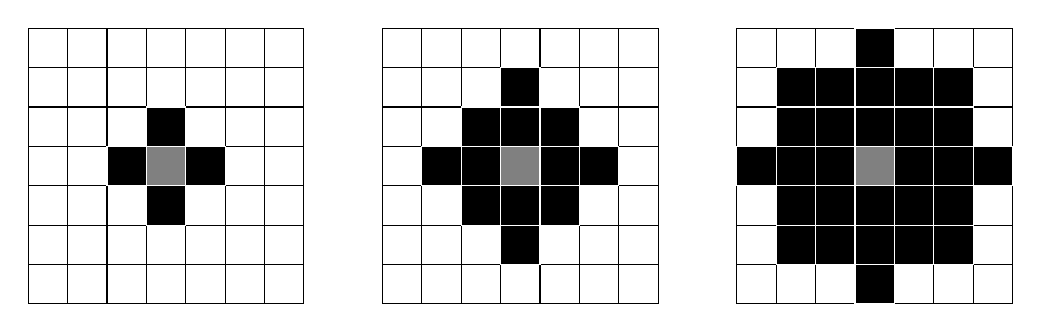
\begin{tikzpicture}[scale=0.5]
        \draw[step=1, black] (0,0) grid (7,7);
        \filldraw[fill=gray, draw=white] (3,3) rectangle (4,4);
        \filldraw[fill=black, draw=white] (3,2) rectangle (4,3);
        \filldraw[fill=black, draw=white] (2,3) rectangle (3,4);
        \filldraw[fill=black, draw=white] (3,4) rectangle (4,5);
        \filldraw[fill=black, draw=white] (4,3) rectangle (5,4);
        
        \begin{scope}[shift={(9,0)}]
            \draw[step=1, black] (0,0) grid (7,7);
            \foreach \i in {1, ..., 9} {
                \pgfmathtruncatemacro\row{mod(\i-1,3)}
                \pgfmathtruncatemacro\col{int((\i-1)/3)}
                \filldraw[fill=black, draw=white] (\row+2,\col+2) rectangle (\row+3,\col+3);
            }
            \filldraw[fill=gray, draw=white] (3,3) rectangle (4,4);
            \filldraw[fill=black, draw=white] (1,3) rectangle (2,4);
            \filldraw[fill=black, draw=white] (5,3) rectangle (6,4);
            \filldraw[fill=black, draw=white] (3,1) rectangle (4,2);
            \filldraw[fill=black, draw=white] (3,5) rectangle (4,6);
        \end{scope}

        \begin{scope}[shift={(18,0)}]
            \draw[step=1, black] (0,0) grid (7,7);
            \foreach \i in {1, ..., 25} {
                \pgfmathtruncatemacro\row{mod(\i-1,5)}
                \pgfmathtruncatemacro\col{int((\i-1)/5)}
                \filldraw[fill=black, draw=white] (\row+1,\col+1) rectangle (\row+2,\col+2);
            }
            \filldraw[fill=gray, draw=white] (3,3) rectangle (4,4); 
            \filldraw[fill=black, draw=white] (0,3) rectangle (1,4);
            \filldraw[fill=black, draw=white] (6,3) rectangle (7,4);
            \filldraw[fill=black, draw=white] (3,0) rectangle (4,1);
            \filldraw[fill=black, draw=white] (3,6) rectangle (4,7);
        \end{scope}
    \end{tikzpicture}
    \caption{Neighbors logic for $r=(1,2,3)$}
    \label{fig:neighbors}
\end{figure}

%Formal definition of a neighbors set $N$ for all of grid boxes $v$, where $V$ is a set of all:
\noindent Formal definition, assuming that grid boxes has resolution (1x1):
\begin{table}[!h]
    \centering
    \begin{tabular}{|c|c|}
        \hline
        Symbol & Description \\
        \hline
        $v_{i,j}$ & Grid box at latitude $i$ and longitude $j$ \\
        $V$  & Set of all grid boxes \\
        $\|v_{m,n} - v_{i,j}\|^2$  & Euclidian distance between centres of $v_{m,n}$ and $v_{i,j}$ \\
        $N_v$ & Set of neighbors for grid box $v$ \\
        \hline
    \end{tabular}
\end{table}
\[
    \forall v_{i,j} \in V: \{\forall v_{m,n \neq i,j} : \|v_{m,n} - v_{i,j}\|^2 \le r\} \in N_{v_{i,j}}
\]

\noindent Unfortunately, the trade-off between memory footprint, computational complexity, and performance gain was not sufficient to incorporate and test bigger $r$ values.

 
 \section{Baselines}
 \subsection{Exponential Smoothing}
 \subsection{Simple Linear Regression}\label{chap:slinear}
 This method is essentially a basic linear regression. When predicting a particular feature $f_i$, each sub-model only considers that specific feature in the input. It is a straightforward approach that assumes no correlation between different features and like any linear regression, it follows the basic assumptions of: linearity, independence, homoscedasticity, normality, absence of multicollinearity, and absence of endogeneity. Given that our task clearly deviates from meeting most of the mentioned assumptions, this method yields results that can be considered fairly average.
\begin{flalign*}
    &\forall f_i \in \mathbf{f}: \hat{y_t}^{f_i} = \Phi_{slr}^{f_i}(X_t^{f_i})\\
    &\hat{Y}_{t} = (\hat{y}_t^{f_1}, ..., \hat{y}_t^{f_n}) \\
\end{flalign*}

 \subsection{Linear Regression}\label{chap:linear}
It follows the same assumptions as \ref{chap:slinear}, but with a tweak. When forecasting the $f_i$ feature, it considers the complete weather state by using all available features as input. This indicate an assumption that different weather features might influence each other. While this approach is still naive linear model, it leads to slightly improved results. \\

  \noindent For both \ref{chap:slinear} and \ref{chap:slinear}, we have examined the performance of basic linear regression, as well as regularized versions - ridge, lasso, and elastic net. The outcomes indicate that ridge regression notably outperforms other methods. Further details are provided in the \ref{chap:report}rd chapter.
\begin{flalign*}
    &\forall f_i \in \mathbf{f}: \hat{y_t}^{f_i} = \Phi_{slr}^{f_i}(X_t)\\
    &\hat{Y}_{t} = (\hat{y}_t^{f_1}, ..., \hat{y}_t^{f_n}) \\
\end{flalign*}
\begin{table}[!h]
    \centering
    \begin{tabular}{|c|c|}
        \hline
        Method & Loss Function \\
        \hline
        Linear & $\sum(y_i - \hat{y_i})^2$ \\
        Ridge & $\sum(y_i - \hat{y_i})^2 + \lambda \sum w_j^2$ \\
        Lasso & $\sum(y_i - \hat{y_i})^2+ \lambda \sum |w_j|$ \\
        Elastic Net & $\sum(y_i - \hat{y_i})^2 +\lambda_1 \sum w_j^2 + \lambda_2 \sum |w_j|$  \\
        \hline
    \end{tabular}
\end{table}
 
 \[
    \mathbf{X} \boldsymbol\beta = \mathbf{\hat{Y}}
 \]

 \[
    \begin{bmatrix}
    x_{11} & x_{12} & \cdots & x_{1n}\\
    x_{21} & x_{22} & \cdots & x_{2n}\\
    \vdots & \vdots & \ddots & \vdots\\
    x_{n1} & x_{n2} & \cdots & x_{nn}
    \end{bmatrix}
    \begin{bmatrix}
    \beta_1\\\beta_2\\ \vdots\\b_n
    \end{bmatrix}
    =\begin{bmatrix}
    \hat{y_1}\\\hat{y_2}\\ \vdots\\\hat{y_n}
    \end{bmatrix}
\]
 \subsection{Gradient Boosting}
Due to the state-of-the-art performance in various tabular data-related challenges and their widespread popularity, we resolve to implement and analyze solutions based on gradient boosting algorithms. We chose two widely used methods, XGBoost ~\cite{Chen_2016} and LightGBM ~\cite{ke2017lightgbm}, both delivering improved results than other baseline methods. The fundamental idea behind gradient boosting lies in the iterative construction of multiple decision trees. Using the gradient boosting algorithm, these trees are generated to improve outcomes and create a more refined representation in each successive iteration. While XGBoost and LightGBM share multiple similarities, the primary distinction lies in their tree construction processes: leaf-wise for XGBoost and level-wise for LightGBM.  \\

\noindent We also explored CatBoost ~\cite{prokhorenkova2019catboost} and classical AdaBoost algorithms. However, due to significantly longer computation times and results that did not surpass other gradient boosting methods, we decided to exclude them from the further experiments and results comparison phase.

\section{Neural network concept}
Optional? \\

\noindent Explain architecture of dense neural networks and other types such as convolutional, recurrent, graph (depending on which one eventually will be used).

\section{GraphCast}
Deep dive into GraphCast architecture.

\section{Neural Network Models}
\subsection{UNet}
This might be consider baseline too but since achieving very high scores and sharing similar characteristics with gnn it might be described here.

\subsection{GNN}
Proposed model architecture and comparision with GraphCast. \\

\noindent After briefly testing multiple Graph Convolutional Cells that support edge feature vectors, we have concluded that the most promising results and sufficient computation time are obtained by TransformerConv ~\cite{shi2021masked}.\\

\noindent Multi-layer perceptron as an embedder converting features dimension into more abstract latent space that stores better representation of weather state.

.... \\

\noindent Multi-layer perceptron as a decoder converting encoded features into its natural representation.


\begin{flalign*}
    X = MLP^{Embedder}(X) \\
    X = GNN_1(X) \\
    ...         \\
    X = GNN_N(X) \\
    \hat{Y} = MLP^{Decoder}(X) \\
 \end{flalign*}

 \begin{flalign*}
    d_{V_i,V_j} &= \sqrt{(V_{j_x} - V_{i_x})^2 + (V_{j_y} - V_{i_y})^2} \\
    e_{V_i,V_j} &= (V_{j_x} - V_{i_x}, V_{j_y} - V_{i_y}, d_{V_i,V_j})
\end{flalign*}

\begin{figure}[!h]
    


\tikzset{every picture/.style={line width=0.75pt}} %set default line width to 0.75pt        

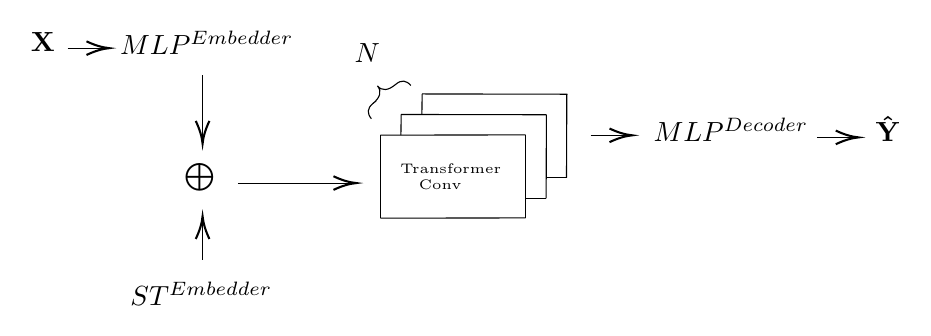
\begin{tikzpicture}[x=0.75pt,y=0.75pt,yscale=-1,xscale=1]
%uncomment if require: \path (0,300); %set diagram left start at 0, and has height of 300

%Shape: Brace [id:dp7019805664018027] 
\draw   (306.33,91) .. controls (304.14,88.39) and (301.74,88.19) .. (299.13,90.38) -- (299.13,90.38) .. controls (295.4,93.52) and (292.44,93.79) .. (290.25,91.18) .. controls (292.44,93.79) and (291.68,96.66) .. (287.95,99.79)(289.63,98.38) -- (287.95,99.79) .. controls (285.34,101.99) and (285.14,104.39) .. (287.33,107) ;
%Straight Lines [id:da24344825121139568] 
\draw    (291.63,114.92) -- (291.63,154.92) ;
%Straight Lines [id:da6110561454804792] 
\draw    (361.7,114.78) -- (361.7,154.78) ;
%Straight Lines [id:da03871795486024654] 
\draw    (291.63,114.92) -- (361.7,114.78) ;
%Straight Lines [id:da49608827752120055] 
\draw    (291.63,154.92) -- (361.7,154.78) ;
%Straight Lines [id:da27192408985546146] 
\draw    (301.69,104.96) -- (371.66,105.08) ;
%Straight Lines [id:da3480819733752343] 
\draw    (301.69,104.96) -- (301.55,114.87) ;
%Straight Lines [id:da3901687935554585] 
\draw    (311.79,95.06) -- (381.76,95.19) ;
%Straight Lines [id:da39197446094452226] 
\draw    (311.79,95.06) -- (311.66,104.98) ;
%Straight Lines [id:da01971233582821519] 
\draw    (371.52,145.35) -- (361.61,145.35) ;
%Straight Lines [id:da8552790800436195] 
\draw    (381.34,135.41) -- (371.43,135.41) ;
%Straight Lines [id:da901598531956911] 
\draw    (371.66,105.08) -- (371.52,145.35) ;
%Straight Lines [id:da7619590199519597] 
\draw    (381.48,95.15) -- (381.34,135.41) ;
%Straight Lines [id:da4912374544292687] 
\draw    (206,175) -- (206,156) ;
\draw [shift={(206,154)}, rotate = 90] [color={rgb, 255:red, 0; green, 0; blue, 0 }  ][line width=0.75]    (10.93,-3.29) .. controls (6.95,-1.4) and (3.31,-0.3) .. (0,0) .. controls (3.31,0.3) and (6.95,1.4) .. (10.93,3.29)   ;
%Straight Lines [id:da3870027998568446] 
\draw    (206,86) -- (206,95) -- (206,117) ;
\draw [shift={(206,119)}, rotate = 270] [color={rgb, 255:red, 0; green, 0; blue, 0 }  ][line width=0.75]    (10.93,-3.29) .. controls (6.95,-1.4) and (3.31,-0.3) .. (0,0) .. controls (3.31,0.3) and (6.95,1.4) .. (10.93,3.29)   ;
%Straight Lines [id:da11332935167733671] 
\draw    (223,138) -- (278,138) ;
\draw [shift={(280,138)}, rotate = 180] [color={rgb, 255:red, 0; green, 0; blue, 0 }  ][line width=0.75]    (10.93,-3.29) .. controls (6.95,-1.4) and (3.31,-0.3) .. (0,0) .. controls (3.31,0.3) and (6.95,1.4) .. (10.93,3.29)   ;
%Straight Lines [id:da8643445648605664] 
\draw    (141,73) -- (159,73) ;
\draw [shift={(161,73)}, rotate = 180] [color={rgb, 255:red, 0; green, 0; blue, 0 }  ][line width=0.75]    (10.93,-3.29) .. controls (6.95,-1.4) and (3.31,-0.3) .. (0,0) .. controls (3.31,0.3) and (6.95,1.4) .. (10.93,3.29)   ;
%Straight Lines [id:da10221146771541123] 
\draw    (502,116) -- (520,116) ;
\draw [shift={(522,116)}, rotate = 180] [color={rgb, 255:red, 0; green, 0; blue, 0 }  ][line width=0.75]    (10.93,-3.29) .. controls (6.95,-1.4) and (3.31,-0.3) .. (0,0) .. controls (3.31,0.3) and (6.95,1.4) .. (10.93,3.29)   ;
%Straight Lines [id:da5913843902335524] 
\draw    (393,115) -- (411,115) ;
\draw [shift={(413,115)}, rotate = 180] [color={rgb, 255:red, 0; green, 0; blue, 0 }  ][line width=0.75]    (10.93,-3.29) .. controls (6.95,-1.4) and (3.31,-0.3) .. (0,0) .. controls (3.31,0.3) and (6.95,1.4) .. (10.93,3.29)   ;

% Text Node
\draw (300,124) node [anchor=north west][inner sep=0.75pt]  [font=\tiny] [align=left] {\begin{minipage}[lt]{28.82pt}\setlength\topsep{0pt}
\begin{center}
{\tiny Transformer }\\{\tiny Conv}
\end{center}

\end{minipage}};
% Text Node
\draw (278,69.4) node [anchor=north west][inner sep=0.75pt]    {$N$};
% Text Node
\draw (170,184.4) node [anchor=north west][inner sep=0.75pt]    {$ST^{Embedder}$};
% Text Node
\draw (165,63.4) node [anchor=north west][inner sep=0.75pt]    {$MLP^{Embedder}$};
% Text Node
\draw (422,105.4) node [anchor=north west][inner sep=0.75pt]    {$MLP^{Decoder}$};
% Text Node
\draw (196,127.4) node [anchor=north west][inner sep=0.75pt]    {$\bigoplus $};
% Text Node
\draw (122,64.4) node [anchor=north west][inner sep=0.75pt]    {$\mathbf{X}$};
% Text Node
\draw (529,104.4) node [anchor=north west][inner sep=0.75pt]    {$\mathbf{\hat{Y}}$};


\end{tikzpicture}


    \caption{Architecture overview}
    \label{fig:architecture}
\end{figure}

\subsection{Additional techniques and feature engineering}\label{chap:feat_eng}
Present concept of spatial-mapping, edge attributes. Explain spatial and temporal feature encodings as well as usage of constants like geopotential. 

%% \subsubsection{Constant features}
\subsubsection{Spatio-Temporal embedder}
To build a better representation of the knowledge of the weather conditions, constant/exogenous features such as geopotential, and land-sea mask were also used as a model input. In addition, with the help of the so-called Spatio-Temporal embedder - $ST^{Embedder}$, we encoded spatial and temporal information, and concatenated it in the process of forward propagation with the input feature tensor, thus obtaining a better knowledge representation for individual grid-boxes. \\

\noindent The encodings for latitude and longitude (lat,lon) of each grid box / node $v_{i,j}$ are represented as:
\[
\mathbf{u}_{geo, v_{i,j}} =
\begin{bmatrix}
    \sin{2\pi\frac{lat}{180}} &
    \cos{2\pi\frac{lat}{180}} &
    \sin{2\pi\frac{lon}{360}} &
    \cos{2\pi\frac{lon}{360}}
\end{bmatrix}
\]

\noindent Encoding of time for entire model input at timestamp $t$, where $(d, h)$ represents the day of the year and the hour in a day, is given by:
\[
\mathbf{u}_{time,t} =
\begin{bmatrix}
    \sin{2\pi\frac{d}{365}} &
    \cos{2\pi\frac{d}{365}} &
    \sin{2\pi\frac{h}{24}} &
    \cos{2\pi\frac{h}{24}}
\end{bmatrix}
\]

\noindent In the subsequent analysis, we denote the product of latitude and longitude spans as $S$. It represents the flattened spatial dimension of tensors. $B$ stands for the batch size. \\ 

\noindent The concatenation of spatio-temporal features with weather features occurs right after the input tensor passes through the $MLP^{Embedder}$ and before entering graph cells. Following the dense layer, weather representation tensor has dimensions ($B$, $S$, hidden), the $\mathbf{u}_{time}$ tensor (batch, 1, 4), and the $\mathbf{u}_{geo}$ tensor ($B$, $S$, 4). To align the corresponding dimensions of $\mathbf{u}_{time}$ it goes through another dense layer with hidden size: $S$, from which it comes out having shape: ($B$, 1, $S$), after transposing the last two dimensions we will get ($B$, $S$, 1) and ability to concatenate all 3 tensors together creating one with shape: ($B$, $S$, hidden+4+1). The concatenated tensor passes through one more dense layer ultimetaly achieving the dimension ($B$, $S$, hidden') and creating a tensor aware of spatio-temporal context. Then, the forward propagatation through the graph cells of the network occurs.

\begin{center}
    \begin{tabular}{|l|l|}
        \hline
        \textbf{Operation} & \textbf{Output shape} \\
        \hline
        $X = MLP^{Embedder}(X)$ & $(B, S, \text{Hidden})$ \\
        $\mathbf{u}_{time} = Dense(\mathbf{u}_{time})^T$ & $(B, S, 1)$ \\
        $X = (X \oplus \mathbf{u}_{time} \oplus \mathbf{u}_{geo})$ & $(B, S, \text{Hidden} + 4 + 1)$ \\
        $X = Dense(X)$ & $(B, S, \text{Hidden'})$ \\
        \hline
    \end{tabular}
\end{center}

\subsubsection{Spatial-Mapping}
Spatial mapping was introduced to extinguish the influence of areas near the boundaries of the input space, which were detrimental to the quality of the prediction. In the original GraphCast architecture, the data spanned the enitre globe, creating a fully connected graph; where our model utilizes data from only a small part of the globe. As the result, vertices located on the space boundaries are connected only to the inner vertices, leading to lack of weather information. Hence, we decided that in the process of training, specifically in cost function computation, and model evaluation only a subspace of the model input is employed. The concept is illustrated in the figure, actual input dimensions are maintained.

\begin{figure}[!h]

\includegraphics[]{figures/spatial_mapping.png}
\caption{A: (32x48) Model input; B: (25x45) Mapped Space}
\end{figure}
 

\noindent TODO: Better visualization
\chapter{Report and analysis}\label{chap:report}

\section{Project structure}
\tikzset{every picture/.style={line width=0.75pt}} 
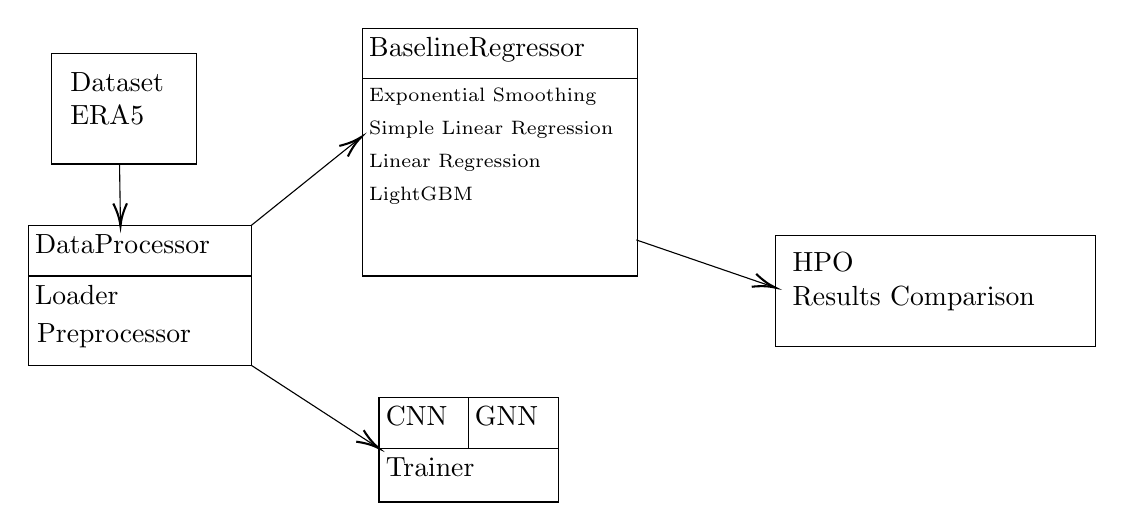
\begin{tikzpicture}[x=0.75pt,y=0.75pt,yscale=-1,xscale=1]
\draw   (49,24) -- (119,24) -- (119,77.4) -- (49,77.4) -- cycle ;
\draw   (38,107) -- (145.47,107) -- (145.47,131.4) -- (38,131.4) -- cycle ;
\draw   (199,12) -- (331.47,12) -- (331.47,36.4) -- (199,36.4) -- cycle ;
\draw   (38,131.4) -- (145.47,131.4) -- (145.47,174.4) -- (38,174.4) -- cycle ;
\draw   (199,36.4) -- (331.47,36.4) -- (331.47,131.4) -- (199,131.4) -- cycle ;
\draw    (82,78) -- (82.42,105.35) ;
\draw [shift={(82.45,107.35)}, rotate = 269.12] [color={rgb, 255:red, 0; green, 0; blue, 0 }  ][line width=0.75]    (10.93,-3.29) .. controls (6.95,-1.4) and (3.31,-0.3) .. (0,0) .. controls (3.31,0.3) and (6.95,1.4) .. (10.93,3.29)   ;
\draw    (145.47,107) -- (196.91,65.65) ;
\draw [shift={(198.47,64.4)}, rotate = 141.21] [color={rgb, 255:red, 0; green, 0; blue, 0 }  ][line width=0.75]    (10.93,-3.29) .. controls (6.95,-1.4) and (3.31,-0.3) .. (0,0) .. controls (3.31,0.3) and (6.95,1.4) .. (10.93,3.29)   ;
\draw   (207,190) -- (293.47,190) -- (293.47,214.4) -- (207,214.4) -- cycle ;
\draw   (207,214.4) -- (293.47,214.4) -- (293.47,240.27) -- (207,240.27) -- cycle ;
\draw    (250.1,190.17) -- (250.1,214.17) ;
\draw    (145.47,174.4) -- (205.32,213.31) ;
\draw [shift={(207,214.4)}, rotate = 213.03] [color={rgb, 255:red, 0; green, 0; blue, 0 }  ][line width=0.75]    (10.93,-3.29) .. controls (6.95,-1.4) and (3.31,-0.3) .. (0,0) .. controls (3.31,0.3) and (6.95,1.4) .. (10.93,3.29)   ;
\draw   (398,112) -- (552,112) -- (552,165.4) -- (398,165.4) -- cycle ;
\draw    (331,114) -- (396.11,136.35) ;
\draw [shift={(398,137)}, rotate = 198.95] [color={rgb, 255:red, 0; green, 0; blue, 0 }  ][line width=0.75]    (10.93,-3.29) .. controls (6.95,-1.4) and (3.31,-0.3) .. (0,0) .. controls (3.31,0.3) and (6.95,1.4) .. (10.93,3.29)   ;
\draw (57,32) node [anchor=north west][inner sep=0.75pt]   [align=left] {Dataset\\ERA5};
\draw (40,110) node [anchor=north west][inner sep=0.75pt]   [align=left] {DataProcessor};
\draw (40,134.4) node [anchor=north west][inner sep=0.75pt]   [align=left] {Loader};
\draw (41,153) node [anchor=north west][inner sep=0.75pt]   [align=left] {Preprocessor};
\draw (201,15) node [anchor=north west][inner sep=0.75pt]   [align=left] {BaselineRegressor};
\draw (201,39.4) node [anchor=north west][inner sep=0.75pt]   [align=left] {{\scriptsize Exponential Smoothing}\\{\scriptsize Simple Linear Regression}\\{\scriptsize Linear Regression}\\{\scriptsize LightGBM}};
\draw (209,193) node [anchor=north west][inner sep=0.75pt]   [align=left] {CNN \ \ GNN};
\draw (209,217.4) node [anchor=north west][inner sep=0.75pt]   [align=left] {Trainer};
\draw (405,119) node [anchor=north west][inner sep=0.75pt]   [align=left] {HPO \\Results Comparison};
\end{tikzpicture}

\section{Dataset description}\label{chap:dataset}
Description of dataset, train, val, test split, resoution of data, generally all details.
\begin{itemize}
    \item Motivation behind usage of GRIB files and their description.
\end{itemize}

\section{Topline}
Description of Tigge - maybe some details about methods that was used to forecast etc.
\section{Preprocessing methods}
Dividing time series into window sequences, normalization techniques

\section{Experiments}
We experimented with various solutions involving different numbers of layers and regularization techniques. Surprisingly, a relatively shallow network consistently outperformed all other solutions. As a result, there was no need to introduce any regularization techniques except LayerNorm, as overfitting was not observed.

\subsection{Hyperparameters optimization}
A short definition of Bayesian optimization and presentation of used Optuna sampler - Tree-Structured Parzen Estimator.~\cite{watanabe2023treestructured} 

\section{Results}
Results presentation, comparision with other models/benchmark scores. Visualisation and analysis.


\begin{table}[ht]
\centering
\caption{Comparison of Model Scores for Each Weather Feature}
\label{tab:model_scores}
\begin{tabular}{lccccc}
\toprule
\textbf{Feature} & \textbf{Metric} & \textbf{Our Model} & \textbf{Tigge} \\
\midrule
\multirow{2}{*}{t2m} & RMSE & 1.566 & \textbf{1.128} \\
                     & MAE  & 1.175 & \textbf{0.826}\\
\midrule
\multirow{2}{*}{sp}  & RMSE & \textbf{1.229} & 3.237  \\
                     & MAE  & \textbf{0.899} & 1.718  \\
\midrule
\multirow{2}{*}{tcc} & RMSE & 0.291 & \textbf{0.251}  \\
                     & MAE  & 0.195 & \textbf{0.150} \\
\midrule
\multirow{2}{*}{u10} & RMSE & 1.145 & \textbf{0.708}  \\
                     & MAE  & 0.830 & \textbf{0.514}  \\
\midrule
\multirow{2}{*}{v10} & RMSE & 1.136 & \textbf{0.696}  \\
                     & MAE  & 0.820 & \textbf{0.502} \\
\midrule
\multirow{2}{*}{tp}  & RMSE & \textbf{0.295} & 1.400  \\
                     & MAE  & \textbf{0.078} & 0.460 \\
\bottomrule
\end{tabular}
\end{table}

\[
\text{RMSE} = \sqrt{\frac{1}{n} \sum_{i=1}^{n} (y_i - \hat{y}_i)^2}
\]

\[
\text{MAE} = \frac{1}{n} \sum_{i=1}^{n} |y_i - \hat{y}_i|
\]

\section{Practical details}
Explain training, evaluating and forecasting details and methods - e.g. spatial mapping of neural nets;
normalization and regularization techniques, used metrics and objectives, post processing, computation time, software and hardware stack etc. 

\chapter{Application}

\section{Overview}
The MeteoMind (nazwa do zmienienia/wywalenia) application is a user-friendly and intuitive tool designed for Android devices. Developed using Kotlin in the Android Studio IDE, this application seamlessly integrates with a powerful neural network model to provide accurate and reliable weather predictions. The core functionality revolves around connecting to an API that houses the neural network model, allowing users to access cyclically generated, future weather forecasts with ease. Application works for devices that run at least Android 11 and newer. Internet connection is required for the app to work properly and it is recommended to allow access to device's location for improved user experience

\section{Functionality}



\section{API}

The API is composed of two endpoints: "/weather" and "/maps". The first request type takes two parameters; longitude and latitude of desirable location that we want obtain the weather to. Despite having data with the precision up to .25 degrees, the API can return the result for any given variables (within the range 55$^{\circ}$N 14$^{\circ}$E to 49$^{\circ}$N 25$^{\circ}$E), thanks to applied bi-linear interpolation. 

    \begin{lstlisting}[language=json, caption={Example of returned JSON with one timestamp}]
    {
      "lat": 49.7128,
      "lng": 21.006,
      "timestamps": [
        {
          "timestamp": "0",
          "values": {
            "sp": 957.9060612843749,
            "tcc": 0.9283748895462038,
            "tp": 0.3892263389520347,
            "u10": 2.7855365757220403,
            "v10": -11.211292881364743,
            "t2m": 9.181962833935547
          }
        }
      ]
    }
    \end{lstlisting}

The "maps" endpoint sends as a response compressed directory that contains colormaps for three features, total precipitation, total cloud cover and 2 metre temperature as well as legend for each one of them that shows the scale of values. 

\begin{figure}[!ht]
\centering
\includegraphics[scale=0.2]{figures/api_maps/t2m0.png}
\includegraphics[scale=0.1]{figures/api_maps/t2m_legend.png}
\includegraphics[scale=0.2]{figures/api_maps/tp0.png}
\includegraphics[scale=0.1]{figures/api_maps/tp_legend.png}
\includegraphics[scale=0.2]{figures/api_maps/tcc0.png}
\includegraphics[scale=0.1]{figures/api_maps/tcc_legend.png}
\caption{Maps and legends for t2m, tp and tcc}
\label{fig:api_maps}
\end{figure}

The API performs also simple preprocessing on the predictions of the model like converting units on total precipitation feature from meters to milimeters and meters per second to kilometers per hour on 10m u- and v- wind components.

\section{Data Storage and DevOps solutions}

\chapter{Conclusions}
\section{Conclusions}
One of the main goals of the thesis was to introduce and compare the performance of several machine learning methods concerning the weather forecasting task and to prove the hypothesis that these methods are promising in the context of future research. We believe that we have succeeded in this goal, in fact, we were even surprised by the quality of some solutions. Unexpectedly, even very naive methods, such as ridge regression, return satisfactory results. Another goal that we successfully achieved was the implementation of a model based on graph neural networks, which, proved to be very light and leverage a small number of parameters, which was not a part of our initial objective. Its results definitely beat other methods and approached the overall performance of an arbitrarily chosen topline, while beating it on features related to pressure and precipitation. This is yet another indication that MLWP methods will be crucial in future approaches to the weather forecasting. Analyses of the quality of solutions depending on the length of the input sequence and the predicted one have confirmed our hypotheses, and recently we have even managed to improve the predictive performance of the topline using a linear combination of its predictions with those returned by our graph architecture.

Limitations associated with the top-performing model, are related to its dissatisfactory predictive capabilities in terms of forecasting on features with challenging distributions, i.e. total precipitation and cloud cover.

\section{Future perspectives}
Future enhancements may include refining the graph architecture structure by integrating additional components previously mentioned in the literature review section. An illustrative approach may be the incorporation of fine-tuning with the autoregressive objective function, similar as was the case for FourCastNet (Section \ref{sec:fourcastnet}). 


Reconstructing our entire training pipeline so that the autoregressive optimization process would be performed at every training step also seems reasonable and worth analyzing. 


Detailed research in the area related to transformer-based architectures is also encouraging, as a suggestion we propose the usage of Vision Transformer as presented in MetNet to enrich our spatial context. Another idea might be to incorporate the ability of recurrent neural networks or attention mechanism to build even better temporal representation. 


It also seems an interesting idea to perform further experiments in the context of creating hybrid models from the solutions we have already implemented -- one might be to combine models with low correlation to form ensembles and see how such a solution would perform. 

Retraining and evaluating implemented solutions, while excluding features with challenging distributions, also seems natural. An interesting experiment would be to remove hard-to-predict features, such as total cloud cover and total precipitation, from the dataset. Since forecasting these variables is difficult, omitting them might yield better results for predicting other features.

In addition, in the case of gaining access to sufficient computing resources, we would be eager to test our architecture and the entire framework for analyzing its behavior for data from a period of more than one year and also from larger boundaries than those covering the administrative area of Poland. It is worth noting that increased computational power would also enable the prediction of additional features and extreme weather conditions.

It would be worth comparing the quality of predictions based on the prediction hour, not just the month. Finally, we believe training and evaluating the models using a more granular interval between timestamps, for example every 1 or 2 hours, would be an interesting analysis.


%--------------------------------------
% Literatura
%--------------------------------------

\bibliographystyle{plain}{\raggedright\sloppy\small\bibliography{bibliography}}

%--------------------------------------
% Dodatki
%--------------------------------------

% \cleardoublepage\appendix%
% \newpage
% \input{chapters/zalacznik.tex}

%--------------------------------------
% Informacja o prawach autorskich
%--------------------------------------

\ppcolophon

\end{document}
